\section{Análisis de la obra pictórica: Lamentación sobre Cristo muerto de Andrea Mantegna}

\begin{figure}[ht!]
	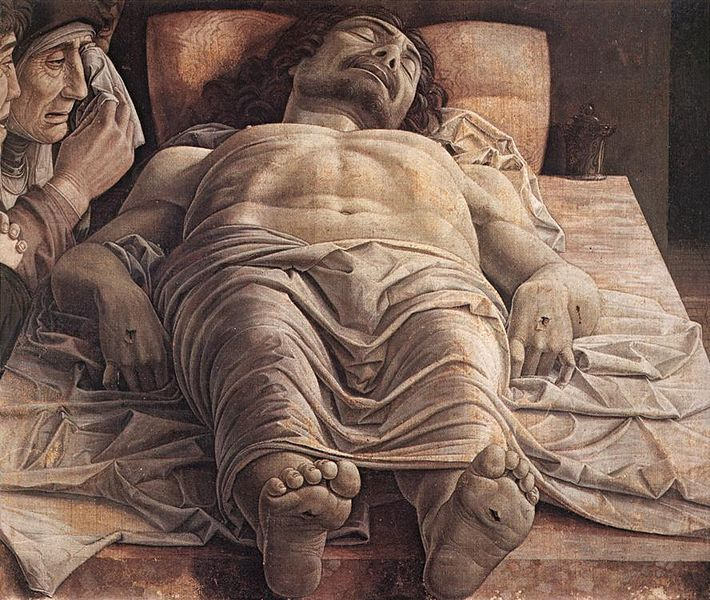
\includegraphics[width=\textwidth]{mantegna.jpg}
   .\caption{Lamentación sobre Cristo muerto de Andrea Mantegna. Pinacoteca de Brera.} % URL: smcarq.blogspot.com.es/2011/07/andrea-mantegna-lamentacion-sobre.html}
\end{figure}

\newpage

%Arte, estilo: Renacimiento italiano, quattrocento
%Cronología: 1480
%Lugar: Pinacoteca de Brera, Milán
%Autor: Andrea Mantegna
%Título: Lamentación sobre Cristo muerto
\begin{description}
\item[Estilo] Renacimiento italiano, Quattrocento
\item[Cronología] 1480
\item[Lugar] Pinacoteca de Brera, Milán
\item[Autor] Andrea Mantegna
\item[Título] Lamentación sobre Cristo muerto
\end{description}

%Función:
\textbf{Contexto histórico:}

Andrea Mantegna realiza esta obra en pleno período humanista, el centro del mundo ya no es Dios o la religión, sino que el hombre pasa a ser el centro. Esto derivaría en ideas de libertad, rivalidad, competencia, que no hacen otra cosa que contribuir al gran avance que se da en el arte durante el Renacimiento en general.

Es durante esta época que los pintores comienzan a tomar importancia como artistas, no solamente como meros técnicos. A partir de este momento empiezan a estudiar formas de hacer las obras más cercanas y reales para el espectador, se busca la consecución de una imagen con volumen, profundidad y dimensiones adecuadas. De esta manera se dan verdaderos progresos en la perspectiva o en las proporciones.

La obra analizada es, de hecho, una obra pionera en la perspectiva con la que representa a Cristo muerto. En épocas anteriores y en otras obras de la misma época en las que se representa a Cristo muerto, lo corriente era contemplarlo de perfil. En la búsqueda de realismo en su obra el autor ladea la cabeza y los pies de la figura, eliminando, de esta forma, la estaticidad que le aporta la simetría del cuerpo, la cual también se ve anulada mediante las arrugas de tela que cubren la pelvis y las piernas de Cristo y las formas laxas del cuerpo.

%TODO Dividir la frase del párrafo en más frases... Es larguísima!
Se trata de una obra dramática del cuerpo de Cristo muerto, antes de la resurrección y el triunfo sobre la muerte. Este dramatismo se percibe en la expresión tanto de la cara de la figura principal, como los rostros de aquellos que contemplan con horror la escena. Y se incrementa con los colores utilizados, de la misma gama cromática, la austera decoración del resto de la estancia, en la que solo vemos la lápida en la que se encuentra tumbado Cristo y la almohada en la que apoya la cabeza.

%http://www.arteespana.com/quattrocentoitaliano.htm
%http://www.arteespana.com/andreamantegna.htm
%http://www.artehistoria.jcyl.es/v2/obras/4376.htm
%http://educacion.ufm.edu/andrea-mantegna-lamentacion-sobre-cristo-muerto-oleo-sobre-tela-en-torno-a-1480-1490/
%http://cv.uoc.edu/~04_999_01_u07/percepcions/perc57.html
%Libro de Olatz


\vspace{12pt}
\textbf{Anatomía de superficie:}

Andrea Mantegna sorprende en su época con esta obra en la que Cristo se presenta en una perspectiva nunca antes vista, y con una figura de proporciones y anatomía exquisitas. Debido precisamente a la perspectiva en la que se encuentra la figura no es fácil discernir el modelo proporcional que sigue, aunque si es apreciable la armonía en la proporción de la figura, con una cabeza adecuada al tamaño del resto del cuerpo.

En esta obra se aprecia de manera sublime la muerte de Cristo. La laxitud de los músculos de las extremidades y la lividez que presenta el cuerpo nos da una idea bastante acertada de la imagen de un cadáver. La palidez amarillenta con la que el autor refleja el cuerpo y los tonos grisáceos incluso amoratados hacen visible lo que se denomina el \textit{pallor mortis}. Esta es una de las fases que acontece a nuestro cuerpo una vez el corazón deja de bombear sangre y, por tanto, esta no llega a los capilares, produciendo una palidez cadavérica. Una vez la sangre deja de circular tiende a por gravedad a dirigirse a la parte baja del cuerpo, que en el caso de la figura de la obra sería en su zona dorsal. En la obra se aprecian zonas más oscuras que podrían coincidir con estas zonas amoratadas del \textit{livor mortis}, pero podrían, de igual manera, tratarse de la propia sombra que proyecta la figura.

Se contemplan los orificios creados por los clavos en primer plano, tanto en los pies como en las manos, representados con gran realismo por el autor. Se pueden observar estos según las creencias de la época en las palmas de las manos, en lugar de a la altura de las muñecas, donde de acuerdo con la creencia actual, eran introducidos.
Las heridas, tanto las originadas por los clavos como la producida por la lanza, se encuentran limpias y sin una gota de sangre. Tanto es así que la del costado derecho apenas es visible en la perspectiva de la figura.

Se puede apreciar sin esfuerzo el volumen de las distintas partes del cuerpo que el autor plasma duramente, casi a modo escultórico. 

Se percibe la distensión de todos los músculos del cuerpo muerto, pudiendo, además, observar estructuras que en obras tan antiguas no solían aparecer, como son las plantas de los pies, donde apreciamos diversas estructuras anatómicas: el arco plantar, claramente definido y el calcáneo y las cabezas de los metatarsianos, que están cubiertos por grasa subcutánea que sirve de almohadillamiento.

También se perfila de forma aparente la caja torácica, tras un vientre hundido, que hace notable el borde costal inferior. Y aunque las estructuras no están claramente representadas se puede intuir, debido al vientre hundido, la espina ilíaca en ambos costados de la pelvis.

Además de estructuras óseas se observan ciertos músculos que recubren tanto la cavidad abdominal como la torácica.

En la porción abdominal, se encuentra, aunque no muy definido, el músculo recto del abdomen y el oblicuo externo, que es el músculo más superficial de los músculos laminares.

En la porción torácica el autor refleja los músculos pectorales y superficialmente incluso identifica los pezones. Sin embargo, da la sensación de que estos músculos tienen la inserción humeral más distal de lo anatómicamente preciso teniendo en cuenta que en realidad insertan cerca de la epífisis del húmero, formando simplemente, el pliegue axilar anterior. Esta sensación puede ser debida a un problema de perspectiva. Otro defecto que podemos observar en la anatomía de este Cristo fallecido es la posición de los hombros con respecto al tronco, estando más ``caídos" de lo que podríamos ver a una persona en la misma posición y desde la misma perspectiva, dejando a la vista un torax en apariencia hinchado. Este tórax hinchado no podría deberse al estado de descomposición en el que se encuentra la figura, puesto que la hinchazón del cuerpo causada por los gases producidos por las bacterias que se encuentran en éste se produce en un estado más avanzado de descomposición.

Las extremidades superiores caen inertes a ambos lados de la figura, con cierta flexión en las articulaciones del codo, muñeca, metacarpofalángicas e interfalángicas probablemente debido al \textit{rigor mortis}. Éste se define como la rigidez que adquieren los músculos tras varias horas de la muerte debido a cambios químicos en las células del cuerpo. Refiriéndome a este mismo proceso, he de mencionar la rigidez de las piernas, puesto que si tal caso no se diera los pies caerían laxos hacia los lados. El músculo deltoides se puede vislumbrar en todo su esplendor recubriendo la articulación del hombro, pero su delimitación es demasiado firme, pudiendo apreciar claramente donde finaliza éste.
